\chapter{Architecture}

Developed architecture / system design / implementation: 1/3

\begin{itemize}
\item start with a theoretical approach
\item describe the developed system/algorithm/method from a high-level point of view
\item go ahead in presenting your developments in more detail
\end{itemize}


\section{Azure IoT Edge Nix Package}

\section{Sample Application}
For verifying that the \textit{Azure IoT Edge} software behaves correctly
with the given operating system, a sample application was developed. This
containerized sample application sends a randomly generated number, from here
on named \textit{measurement value}, to the \textit{Edge Hub}. The architecture
of how the components interact with each other, was modelled after a real
world \ac{IIoT} application for natural gas measurements. All proprietary
source code and everything else which was subject to copyright and intellectual
property was not used in this research. The application features a \ac{HTTP}
\ac{REST} \ac{API} for further automation. For a complete overview of which
containers the application is compromised, refer to table \ref{tab:containers}.


\begin{table}[H]
    \centering
    \begin{tabular}{ p{0.33\linewidth} p{0.14\linewidth} p{0.45\linewidth}}
        \toprule
        \textbf{Container Name} & \textbf{Developer} & \textbf{Description} \\
        \midrule
        Edge Agent & Microsoft & Application for managing containers and deployments. \\
        Edge Hub & Microsoft & Gateway and buffer for sending messages to cloud services. \\
        Edge Metrics Collector & Microsoft & Application for collecting container logs, metrics and health data. \\
        SQL Server & Microsoft & Containerized instance of Microsoft's SQL server. \\
        sampleapp UI & Elias Frank & Web application for viewing telemetry data from the \ac{API}. \\
        sampleapp API & Elias Frank & \ac{REST} \ac{API} for retrieving telemetry locally for further automation. \\
        sampleapp Telemetry Service & Elias Frank & Background service for randomly generating telemetry. \\
        \bottomrule
    \end{tabular}
    \caption{Sample Application: List of containers}
    \label{tab:containers}
\end{table}

The sections \ref{sec:telemetry-service}, \ref{sec:api}, \ref{sec:ui} further
describe the functionalities of the individual applications that form together
the entire sample application.

\subsection{sampleapp Telemetry Service} \label{sec:telemetry-service}
The \textit{sampleapp Telemetry Service} is an application developed for this
research. The application has the following main functionalities:

\begin{itemize}
    \item It sends the current timestamp to the \textit{Edge Hub} on start up,
    \item It sends a randomly generated telemetry value to the
    \textit{Edge Hub} every minute,
    \item It stores the telemetry value in a \ac{SQL} database,
    \item It sends the current uptime of the application to the \textit{Edge Hub}
    every hour.
\end{itemize}
The \textit{sampleapp Telemetry Service} is written in \textit{C\#} using the
\textit{ASP.NET} framework and the \textit{Azure Device} \ac{SDK}.

\subsection{sampleapp API} \label{sec:api}
The \textit{sampleapp API} is a \ac{HTTP} \ac{REST} \ac{API} developed for this
research. The application has the following main functionalities:

\begin{itemize}
    \item Retrieve telemetry values from the \ac{SQL} database via an
    \ac{REST} endpoint,
    \item Enables customers to connect automation from their local network.
\end{itemize}
The \textit{sampleapp API} is written in \textit{C\#} using the \textit{ASP.NET}
framework and the \textit{Entity Framework Core} for database access.

\subsection{sampleapp UI} \label{sec:ui}
The \textit{sampleapp UI} is a web application developed for this research.
The application has the following main functionalities:

\begin{itemize}
    \item
\end{itemize}
The \textit{sampleapp UI} is written in \textit{C\#} using the \textit{ASP.NET}
framework and the \textit{Blazor Web Assembly} framework for \textit{.NET}.

\begin{figure}[H]
    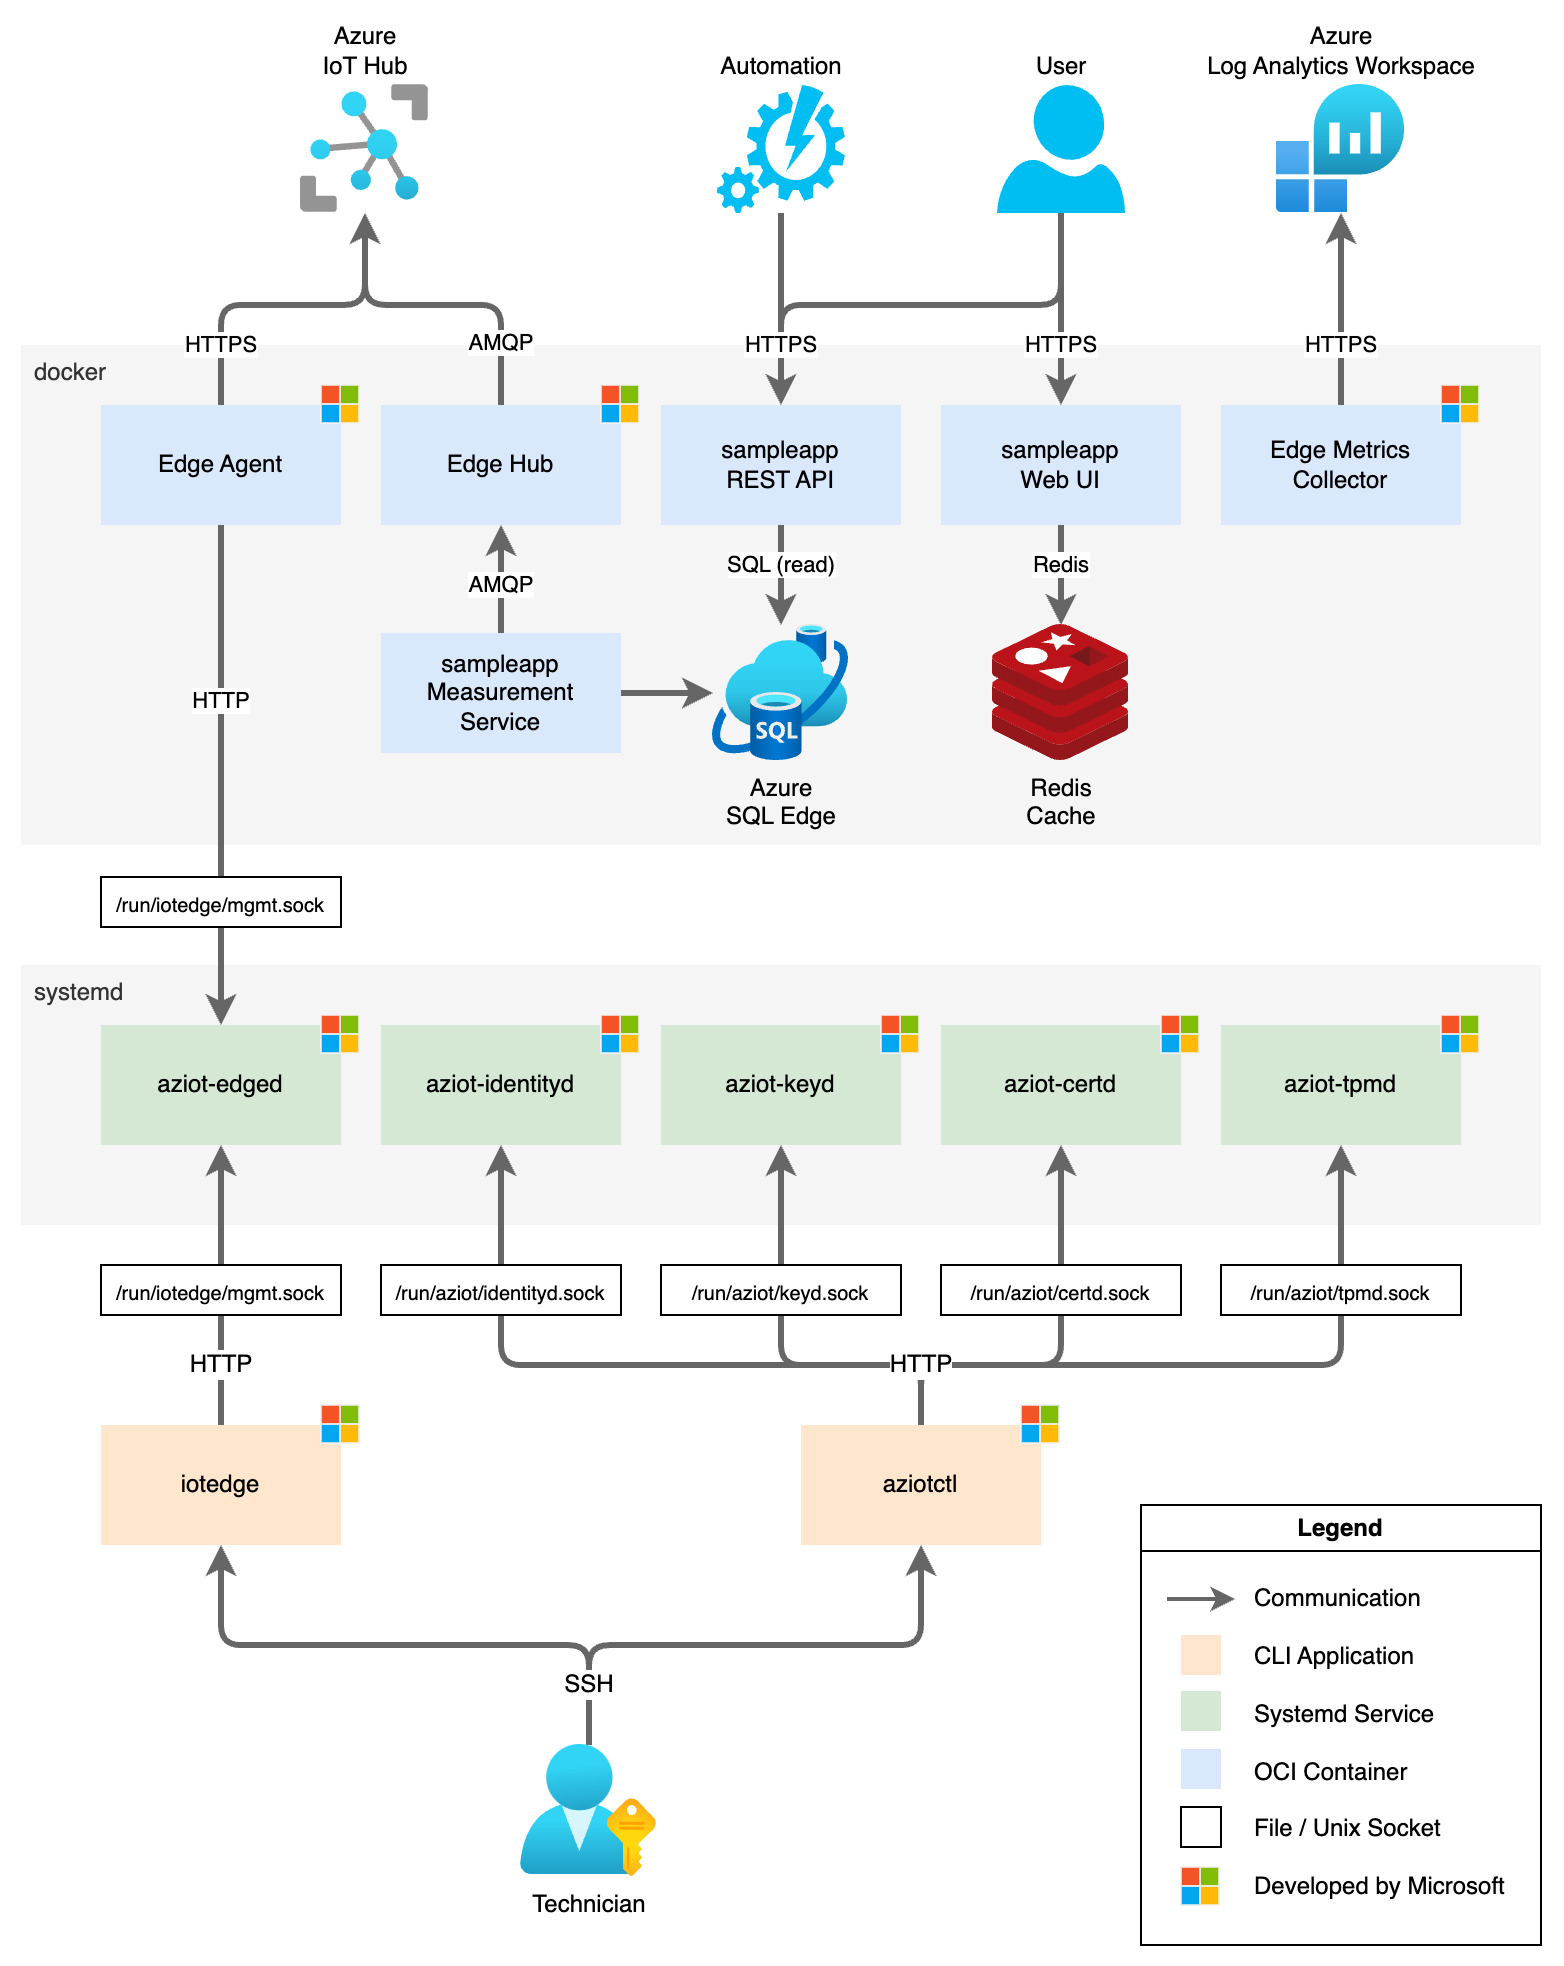
\includegraphics[width=\textwidth]{fig/sample-app-dataflow.drawio.png}
    \caption{Sample Application: Architecture Overview}
    \label{fig:sample-app-architecture}
\end{figure}


\begin{table}[H]
    \centering
    \begin{tabular}{l l l l }
        \toprule
        \textbf{From} & \textbf{To} & \textbf{Port} & \textbf{Protocol} \\
        \midrule
        sampleapp Telemetry Service & Edge Hub & C & D \\
        sampleapp Telemetry Service & SQL Server & C & D \\
        Edge Metrics Collector & Edge Agent & 9000 & \ac{HTTP} \\
        Edge Metrics Collector & Edge Hub & 9000 & \ac{HTTP} \\
        Edge Metrics Collector & sampleapp API & 8080 & \ac{HTTP} \\
        Edge Metrics Collector & sampleapp Telemetry Service & 8080 & \ac{HTTP} \\
        \bottomrule
    \end{tabular}
    \caption{Sample Application: Communication table}
\end{table}

\section{Experiments}
\subsection{Verifying the correctness of Azure IoT Edge}
For verifying that \textit{Azure IoT Edge} was correctly installed
and behaves according the expected functionality on the given
\ac{OS}, a number of criteria where chosen. They represent the registration
of a single device according to Microsoft's documentation, but further
invoke the health checks of the Sample Application's components.
The criteria are as follows:

\begin{enumerate}
    \item The \code{iotedge} \ac{CLI} is in the path.
    \item A configuration file can be generated with \code{iotedge config}.
    \item The device can be registered with \code{iotedge config apply}.
    \item \code{iotedge check} reports no errors.
    \item \code{iotedge list} reports that the following containers
    are running:
    \begin{itemize}
        \item edgeAgent
        \item edgeHub
        \item IotEdgeMetricsCollector
        \item sql-server
        \item sampleapp-telemetry-service
        \item sampleapp-api
        \item sampleapp-ui
    \end{itemize}
    \item \code{curl localhost:8001} returns "Healthy".
    \item \code{curl localhost:8002} returns "Healthy".
    \item Device messages are visible in the cloud using the \textit{Azure IoT Explorer}.
\end{enumerate}
These checks must be performed on all the \ac{OS}s, for a direct comparison.
They serve as a baseline for all further experiments, because all further
experiments are building on the assumption that \textit{Azure IoT Edge} was
installed and is behaving correctly.

\subsection{Image size}
When updating the operating system with an A/B failover model, the entire
image needs to be downloaded and written to a secondary partition. In this
\ac{OTA} scenario the size of the operating system image is critical.
For this experiment two sizes are relevant, when comparing operating systems.
Firstly, the actual size of the image that needs to be written to the partition.
Secondly, the size that the entire system takes up on the disk after booting.

\subsection{Boot times}
Customers of certain industries require high availability and reliability for
their \ac{IIoT} devices and applications. These availability requirements
are commonly legally and formally negotiated in \ac{SLA}s between
the customer and a service provider \cite{msdoc-slas}.

An important consideration for service providers to achieve high
availability is the boot time of the \ac{OS}. However for this experiment the
time until operability is considered, instead of the actual boot time of the
\ac{OS}. The time until operability is more relevant for service providers
when defining \ac{SLO}.
For this experiment an outage of the service will be simulated by sending a
\textit{reboot} system call to the kernel with the \textit{reboot}
command line tool. It is important to note, that the "--force" option will
instruct the command line tool to not call the \textit{shutdown} system call,
which results in a faster shutdown of the system \cite{man-reboot}\cite{man-shutdown}.
Just before the system is rebooted, the current time will be printed.
\\

\begin{lstlisting}[caption=Command to print the current time and reboot]
date +%s && reboot -f
\end{lstlisting}
After the \ac{OS} rebooted and \textit{systemd} has started, the
\textit{Sample Application Telemetry Service} will send the current timestamp
to the \textit{Azure IoT Hub} where it can be retrieved. When comparing
the first timestamp from the shell command with the second timestamp from
the \textit{Azure IoT Hub}, the time until operability can be calculated.
This experiment must be repeated until the standard deviation is low enough
to have a confident mean value for each \ac{OS}.



\section{Build Host}
During the experiments conducted in this thesis, it was
required to compile, package, and build various software.
Also, the operating system variants required a
computationally expensive creation of an installable image.
For building and testing the various operating systems and
software packages the following hardware was used:
\begin{itemize}
    \item Processor: AMD Ryzen 7 5700X,
    \item Memory: 32 GB,
    \item Storage: 512 GB SSD,
\end{itemize}

Further, the following software versions were used on the build host:
\begin{itemize}
    \item Linux 6.5.6,
    \item Git 2.42.0,
    \item Nix 2.18.1,
    \item GCC 13.2.1 20230801,
    \item Make 4.4.1.
\end{itemize}
